% single-column 'preprint' layout for submission; change preprint -> reprint for the two-column look
\documentclass[aps,pra,preprint,superscriptaddress,amsmath,amssymb]{revtex4-2}
\usepackage[utf8]{inputenc}
\usepackage[T1]{fontenc}
\usepackage{graphicx}
\usepackage{url}
\usepackage{newunicodechar}
\usepackage{lineno}   % line numbers, as in the APS sample manuscript
\newunicodechar{§}{\S}
\newunicodechar{²}{\ensuremath{^{2}}}
\newunicodechar{³}{\ensuremath{^{3}}}
\newunicodechar{·}{\ensuremath{\cdot}}
\newunicodechar{¹}{\ensuremath{^{1}}}
\newunicodechar{½}{\ensuremath{\tfrac{1}{2}}}
\newunicodechar{×}{\ensuremath{\times}}
\newunicodechar{Δ}{\ensuremath{\Delta}}
\newunicodechar{Σ}{\ensuremath{\Sigma}}
\newunicodechar{α}{\ensuremath{\alpha}}
\newunicodechar{β}{\ensuremath{\beta}}
\newunicodechar{δ}{\ensuremath{\delta}}
\newunicodechar{ζ}{\ensuremath{\zeta}}
\newunicodechar{κ}{\ensuremath{\kappa}}
\newunicodechar{μ}{\ensuremath{\mu}}
\newunicodechar{ν}{\ensuremath{\nu}}
\newunicodechar{ρ}{\ensuremath{\rho}}
\newunicodechar{σ}{\ensuremath{\sigma}}
\newunicodechar{τ}{\ensuremath{\tau}}
\newunicodechar{†}{\ensuremath{^\dagger}}
\newunicodechar{…}{\ldots{}}
\newunicodechar{′}{\ensuremath{'}}
\newunicodechar{⁰}{\ensuremath{^{0}}}
\newunicodechar{⁴}{\ensuremath{^{4}}}
\newunicodechar{⁵}{\ensuremath{^{5}}}
\newunicodechar{⁶}{\ensuremath{^{6}}}
\newunicodechar{⁹}{\ensuremath{^{9}}}
\newunicodechar{⁺}{\ensuremath{^{+}}}
\newunicodechar{⁻}{\ensuremath{^{-}}}
\newunicodechar{₀}{\ensuremath{_{0}}}
\newunicodechar{₁}{\ensuremath{_{1}}}
\newunicodechar{₂}{\ensuremath{_{2}}}
\newunicodechar{→}{\ensuremath{\to}}
\newunicodechar{−}{\ensuremath{-}}
\newunicodechar{√}{\ensuremath{\surd}}
\newunicodechar{∞}{\ensuremath{\infty}}
\newunicodechar{≈}{\ensuremath{\approx}}
\newunicodechar{≠}{\ensuremath{\neq}}
\newunicodechar{≡}{\ensuremath{\equiv}}
\newunicodechar{≤}{\ensuremath{\leq}}
\newunicodechar{≥}{\ensuremath{\geq}}
\newunicodechar{≳}{\ensuremath{\gtrsim}}
\newunicodechar{⟨}{\ensuremath{\langle}}
\newunicodechar{⟩}{\ensuremath{\rangle}}
\begin{document}
\linenumbers
\title{A screened Rydberg formula for the successive ionization energies of all atoms and ions}
\author{Muhammad Awais}
\email{mawais9171@gmail.com}
\affiliation{Independent researcher, Multan, Pakistan}
\date{\today}
\begin{abstract}
We present a closed-form expression, the \emph{screened Rydberg formula}, for the successive ionization energy IE(Z, N) of any atom or ion. Its inputs are the nuclear charge Z and the ground electron configuration. The formula keeps the hydrogenic form Ry Z\_eff²/n² and splits the effective charge into two parts. The first is the first-order screening constant σ₁ = −n²ΔE₁ of the 1/Z perturbation expansion. It has no adjustable parameter, it is a rational number for every configuration, and we tabulate it for N = 1–110. The second is a fitted higher-order remainder that depends on the ion charge in an Edlén-type form. A saturation construction keeps Z − N + 1 ≤ Z\_eff ≤ Z for any parameter values (given 0 ≤ σ₁ ≤ N − 1, which holds for every configuration we use) and preserves the exact Z² and Z coefficients of the 1/Z series. One-electron Dirac, recoil, finite-nuclear-size and QED corrections enter without fitted parameters. The final model has 33 global parameters and none per element or ion. On the 5847 successive ionization energies in the NIST Atomic Spectra Database (Z = 1–110) its mean absolute percentage error (MAPE) is 1.87 \% (median 0.94 \%). It is 7.52 \% for the first ionization energies of neutral atoms and 0.0012 \% for hydrogen-like ions; the H-like figure agrees with, but is not independent of, the QED theory behind the NIST values. We chose the model with a pre-registered score that never used the extrapolation test, although its interpolation splits contain heavy elements. Fitted on Z ≤ 54 and used to predict Z = 55–110, the model gives 6.60 \% MAPE (median 1.62 \%). On the same rows Slater's rules give 11.6 \%, a published parameter-free screened-hydrogenic model 13.6 \%, and two earlier fitted variants without the bound 57.2 \% and 170 \% (Table I). Heavy neutral atoms remain the weak point, with 21.8 \% MAPE on their first ionization energies in that test. The Z ≤ 54 fit puts Pb and Tl at about 1.2 and 1.7 eV (NIST 7.42 and 6.11 eV) and makes Lr negative, and the all-data fit puts oganesson (3.66 eV) far below radon (NIST 10.75 eV). We report these failures and have not corrected them.
\end{abstract}
\maketitle

\section{Introduction}

The Bohr energy Ry Z²/n² is exact only for a non-relativistic one-electron ion. For every other atom and ion the ionization energy (IE) depends on electron–electron repulsion, which has no closed-form solution for N ≥ 2. Four lines of work bear on the problem.


Slater~\cite{r1} replaced Z by an effective charge Z − σ, with σ given by counting rules fitted by hand to atomic data. Clementi and Raimondi~\cite{r2,r3} obtained σ from optimised self-consistent-field orbital exponents of neutral atoms. Both were designed for orbitals of neutral atoms, not for the full set of successive IEs. Scored as IE formulas on all NIST ions with a total-energy difference, Slater's rules give 11.8 \% MAPE and Clementi–Raimondi 120 \% (Sec. IV).


Layzer~\cite{r4,r5} showed that the non-relativistic energy of a fixed configuration is an asymptotic series E = Z²E₀ + ZE₁ + E₂ + …. E₀ is hydrogenic, and E₁ is a rational combination of hydrogenic Slater integrals, which fixes the Z → ∞ limit of the screening constant exactly. Higher orders need continuum sums~\cite{r6,r7}. Along isoelectronic sequences, Edlén~\cite{r8} described the smooth variation of screening with ion charge by expansions in 1/(ζ + s). Z-expansion codes with relativistic corrections were developed for selected sequences~\cite{r9}.


Screened hydrogenic models (SHMs), starting with Mayer~\cite{r10} and More~\cite{r11}, are used in plasma-physics codes. Their screening constants have been tabulated or fitted with l-splitting~\cite{r12,r13}, derived from analytical potentials~\cite{r14,r15}, fitted by a genetic algorithm with relativistic subshells~\cite{r16}, or computed self-consistently as functions of Z and N without parameters~\cite{r17,r18,r19,r20,r21,r22}. Average-atom and kinetics codes use SHMs because they are fast and cover all ions~\cite{r23,r24,r25}.


Ab initio methods give more accurate numbers: Koopmans' theorem~\cite{r26}, ΔSCF Hartree–Fock and Kohn–Sham DFT~\cite{r27,r28}, correlated non-relativistic energies~\cite{r29}, and Dirac–Fock total energies for all ground configurations up to Z = 118~\cite{r30}. They are numerical procedures, not formulas.


We found no closed-form expression that covers every ion of every element from the configuration alone, reproduces the large-Z behaviour of the 1/Z expansion exactly, reports every fitted parameter, and is validated on all NIST successive IEs with held-out tests fixed in advance, including an extrapolation to heavier elements. The SHM papers we read report accuracy on their fitting data or, like~\cite{r20}, on selected sequences. Scored on our rows (Sec. IV E), the constants of Mendoza et al. give 2.82 \% MAPE on the 5011 rows they cover. This paper addresses that gap. It does not propose a new law of atomic physics, and Sec. V A lists what is rediscovered.


The paper makes four contributions. It tabulates σ₁ for every NIST ground configuration with N = 1–110, as a parameter-free counterpart to Slater's σ that is exact as Z → ∞ (Sec. II A, Sec. IV F). It defines the screened Rydberg formula, σ₁ plus a bounded Edlén-type remainder with 33 global parameters (Secs. II B–II D). It applies one validation protocol, with a pre-registered selection score and a single extrapolation test, to the final model, its ancestors and the published baselines (Sec. III, Sec. IV). And it compares the formula with two published SHMs, re-implemented and scored with the same scorer (Sec. IV E): the parameter-free Kregar/Di Rocco model on all 5847 rows, and the fitted constants of Mendoza et al. (2011) on the 5011 rows they cover.


\section{Theory}

Sec. II A uses atomic units; energies are converted to eV with Ry = 13.6057 eV. Z is the nuclear charge, N the number of electrons before ionization, and Z\_a = Z − N + 1 the charge seen by the departing electron. (n, l) is the removed subshell and k its occupancy.


\subsection{Exact first-order screening from the 1/Z expansion}

Scaling r → ρ/Z turns the non-relativistic Hamiltonian into H = Z²[H₀ + Z⁻¹V], with H₀ hydrogenic and V = Σ 1/ρ\_ij. Rayleigh–Schrödinger perturbation theory in 1/Z then gives, for a fixed configuration and term, E(Z, N) = Z²E₀ + ZE₁ + E₂ + …, and the ionization energy is


\begin{equation}
\mathrm{IE}(Z,N)=Z^2\Delta E_0+Z\,\Delta E_1+\Delta E_2+\dots,\qquad \Delta E_k=E_k(N-1)-E_k(N).
\end{equation}

At zeroth order ΔE₀ = 1/(2n²), which is Bohr's formula. At first order E₁ = ⟨V⟩ over the Z = 1 hydrogenic state. Every hydrogenic radial integral F\textasciicircum{}k and G\textasciicircum{}k is a rational number, because each product P\_a P\_c is a polynomial times e\textasciicircum{}\{−βr\} with rational β; for example F⁰(1s,1s) = 5/8, F⁰(1s,2s) = 17/81 and G⁰(1s,2s) = 16/729. We evaluate the integrals in exact rational arithmetic and combine them with exact angular algebra. For open subshells E₁ is evaluated for the Hund ground term by projecting onto the highest-weight (S, L) subspace. Where hydrogenic degeneracy couples configurations (the Layzer complex, e.g. 1s²2s² with 1s²2p²), V is diagonalised within the complex. For two or more open subshells we use a high-spin coupled term, which is the one approximation in σ₁.


Completing the square in the first two terms defines the first-order screening constant


\begin{equation}
\mathrm{IE}\simeq \Delta E_0\,(Z-\sigma_1)^2,\qquad \sigma_1=-\frac{\Delta E_1}{2\Delta E_0}=-n^2\Delta E_1 .
\end{equation}

σ₁ is Layzer's Z → ∞ screening constant. It has no adjustable parameter and depends on the configuration, not on Z. For He-like ions E₁(1s²) = 5/8, so σ₁(He) = 0.6250 (Slater: 0.30). For Li-like ions E₁(1s²2s) = 5965/5832 = 1.0228052 = 5/8 + 2·17/81 − 16/729, so ΔE₁ = −0.397805 and σ₁ = 1.5912. For Be-like ions the complex value E₁ = 1.5592742 agrees with Layzer's.


The series fails for near-neutral atoms (Sec. IV F), because its expansion parameter is effectively N/Z. For a neutral atom Z − σ is only 1–3, so a 10 \% error in σ becomes a 100–1000 \% error in IE. The higher orders have no closed form: E₂ already requires sums over the hydrogenic continuum. The completed-square guess ΔE₂ = ΔE₁²/(4ΔE₀), for example, is 24–26 \% too large for He- and Li-like ions. For this reason the remainder in Sec. II B is fitted.


\subsection{The screened Rydberg form with a bounded remainder}

The final model (code name pa\_hier\_rel) is


\begin{equation}
\mathrm{IE}(Z,N)=\mu(Z)\Big\{\mathrm{Ry}\,\frac{Z_\mathrm{eff}^2}{n^2}\,F_{n,j}(Z_\mathrm{eff})\Big[1+r_c\,\frac{(Z\alpha)^2}{n}\Big(\frac{Z_\mathrm{eff}}{Z_a}-1\Big)\Big]+\mathrm{Ry}\,\frac{x_l\,K_l(k)}{n^2}\Big\}-\big[\Delta E_\mathrm{QED}+\Delta E_\mathrm{FNS}\big]_{Z,n}\Big(\frac{Z_\mathrm{eff}}{Z}\Big)^2 ,
\end{equation}

where the last term applies only to the removal of an ns electron with n ≤ 2, and


\begin{equation}
Z_\mathrm{eff}=Z-\sigma_1(\mathcal C)-D,\qquad
D=\frac{T}{Z_a+\kappa+|T|/h},\qquad
h=\begin{cases}(N-1)-\sigma_1 & T\ge 0\\ \sigma_1 & T<0\end{cases},\qquad
T=\sum_{g}\tau_g\,\nu_g+\sum_{c}\delta\tau_c\,\nu_c .
\end{equation}

Each of the other N − 1 electrons, in a subshell (n′, l′), is counted in exactly one of five screening groups ν\_g. The group \emph{same} holds the k − 1 other electrons of (n, l). The group \emph{out} holds outer electrons, with n′ > n or with n′ = n and l′ > l. All remaining electrons are inner. For an s or p target, inner electrons with n′ ≥ n − 1 form \emph{in} (the ns electrons of an np target plus the whole (n − 1) shell, including its d and f electrons) and those with n′ ≤ n − 2 form \emph{core}. For a d or f target, every inner electron, from the same-n lower-l subshells down to 1s, is in \emph{df}. Hence Σ\_g ν\_g = N − 1, and each group has a coefficient τ\_g. As (ν\_same, ν\_in, ν\_core, ν\_df, ν\_out), O 2p⁴ gives (3, 4, 0, 0, 0) and Na 3s gives (0, 8, 2, 0, 0). Fe 3d⁶4s² with 4s removed gives (1, 14, 10, 0, 0), because 3d⁶ belongs to the (n − 1) shell. Pb 6p² gives (1, 20, 60, 0, 0), with 6s²5s²5p⁶5d¹⁰ in \emph{in} and every electron with n′ ≤ 4, including 4f¹⁴, in \emph{core}.


The screening classes ν\_c (Table IX) refine the groups. An electron's class depends on the target type (s/p, d or f), on n − n′ and on l′. Each class lies inside one group, and an electron of class c in group g contributes τ\_g + δτ\_c to T. A ridge penalty (10⁻⁴ per row) shrinks the deviations toward their group value. Two of the 21 classes are empty in all 5847 rows and carry no δτ\_c: sn\_out (n′ = n, l′ > l) and out\_sp (n′ > n, s/p target). That leaves the 19 of Table VIII. The bounded 9-parameter variant (pa\_bound9) and the pocket formula (Appendix A) use the five groups without classes. An independent implementation of the rule reproduces the code's group and class counts with 0 mismatches on all 5847 rows and on all 7021 configurations with Z ≤ 118 (\texttt{tools/check\_grouping\_rule.py}).


The removed subshell (n, l) is the one whose occupancy drops from the N-electron configuration to the NIST ground configuration of the (N − 1)-electron ion. The N-electron configuration is the NIST ground configuration, or the Madelung order if the ion is not tabulated. For a rearranging ion (e.g. V 3d³4s² → V⁺ 3d⁴) it is the subshell that loses most electrons, with ties going to larger n and then larger l. If the (N − 1)-electron ion is not tabulated, or the user supplies the configuration, the outermost subshell (largest n, then largest l) is removed.


The Hund term uses K\_l(k) = [P(k) − P(k−1)] − 2l(k−1)/(4l+1), the change in the number of parallel-spin pairs relative to a statistical average. P(k) is the number of parallel-spin pairs of l\textasciicircum{}k under Hund's first rule. Equivalently K\_l(k) = (2l+1)(k−1)/(4l+1) for k ≤ 2l+1 and K\_l(k) = −K\_l(4l+3−k) above half filling, so K\_s ≡ 0, K\_p = 0, 0.6, 1.2, −1.2, −0.6, 0 for k = 1…6, K\_d = (5/9)(0, 1, 2, 3, 4, −4, −3, −2, −1, 0) and K\_f = (7/13)(0, 1, …, 6, −6, …, −1, 0). The amplitude x\_l is fitted for l = p, d, f; s electrons have no Hund term.


Three inputs need a precise definition. σ₁ is evaluated for the \emph{frozen} configuration, the N-electron configuration minus one (n, l) electron, and not for the ground configuration of the ion. The two differ only for the 63 rearranged rows, and the choice keeps ΔE₀ = 1/(2n²) on those rows. The reduced-mass factor is μ(Z) = M/(M + m\_e), where M is the nuclear mass of the isotope used in the QED tabulation~\cite{r31}. The QED and finite-nuclear-size shift is applied only to 1s and 2s removal (427 rows); it is the one-electron shift of Sec. II D for charge Z, scaled by (Z\_eff/Z)², and reaches at most 0.9 \% of the IE (at Z = 110, N = 2). For N = 1, T = 0 and so D = 0.


A reader cannot reconstruct the frozen-configuration σ₁, μ(Z) or the QED/FNS shift from the text alone, so we publish every per-row input in \texttt{results/model\_inputs.csv}: removed subshell, k, j, σ₁, ν\_g, ν\_c, K, μ and QED/FNS. A short script that uses only this table, the equations above and the parameters of Table VIII (\texttt{tools/verify\_from\_inputs.py}, which imports no model code) reproduces the production code on all 5847 rows to 7·10⁻¹⁶ relative, for the final model and for pa\_bound9.


The saturation form of D has two properties for any parameter values. First, it bounds the effective charge, Z\_a ≤ Z\_eff ≤ Z. Writing D = sign(T)·h·u/(1+u) with u = \textbar{}T\textbar{}/[h(Z\_a+κ)] gives \textbar{}D\textbar{} < h, so Z\_eff can fall neither below the fully screened, non-penetrating limit Z\_a nor above the bare charge Z. Because h = (N−1) − σ₁ or σ₁, this requires 0 ≤ σ₁ ≤ N − 1. We have checked rather than proved that condition: it holds for all 7021 ground and Madelung configurations with Z ≤ 118, and the code warns if a user-supplied configuration breaks it. Second, it keeps the exact asymptotics. At fixed N and Z\_a → ∞, D → T/(Z\_a+κ) = O(1/Z), so the expansion of IE begins Ry[Z² − 2Zσ₁ + O(1)]/n² and its Z² and Z coefficients are those of the exact 1/Z series. The fitted part represents only ΔE₂ and higher orders, that is relaxation, correlation and penetration at low ion charge.


\subsection{Charge-dependent penetration as an Edlén-type term}

We found the remainder's dependence on 1/(Z\_a + κ) empirically (docs/semi\_empirical.md). Along every isoelectronic sequence the excess charge p = Z\_eff − Z\_a grows with ion charge q as p∞ − τ/(Z\_a + κ), with one κ for all sequences. For the Na sequence (3s), p = 0.84, 1.15, 1.34, 1.46, 1.56 for q = 0–4 and 2.11 at q = 20. Adding the term reduced the error of the purely fitted model from about 9 \% to about 2 \% MAPE. This is an independent rediscovery of the isoelectronic regularity that Edlén formalised~\cite{r8}, and it is consistent with Layzer's theory, in which the screening constant is σ₀ + σ₁′/Z + …. What is specific here is narrower: one denominator for all sequences, combined with exact σ₁ and with the saturation bound of Sec. II B.


\subsection{Relativistic, recoil, finite-size and QED corrections}

F\_\{n,j\}(ζ) is the exact ratio of the point-nucleus Dirac binding energy to the Schrödinger energy for charge ζ. With x = ζα and κ = j + ½, F = (2n²/x²)·\{1 − [1 + (x/(n − κ + √(κ² − x²)))²]\textasciicircum{}(−1/2)\}. j follows jj filling, l − ½ while k ≤ 2l and l + ½ otherwise. We write F to avoid confusion with the screening remainder D.


The bracket 1 + r\_c(Zα)²(Z\_eff/Z\_a − 1)/n is a Fermi–Segrè-type correction for the penetration of the valence electron into the region of full nuclear charge. Its five coefficients r\_c, for the classes s, p½, p3/2, d and f, are fitted.


For one-electron ions we use the Dirac energy with a numerically solved finite-nuclear-size (FNS) shift, Barker–Glover recoil, the Uehling vacuum polarisation computed over the Dirac 1s density, and the one-loop self-energy function F\_SE(Zα) from the all-order tabulation of Yerokhin and Shabaev~\cite{r31}. The 2 × 110 tabulated values are external theory inputs, not fitted parameters. In the many-electron formula the QED and FNS shifts are applied only to 1s and 2s removal, scaled by (Z\_eff/Z)². The closed-form low-order Zα expansion of F\_SE cannot replace the table: it matches the table at Z = 1 but diverges for Z ≳ 15, and it gives 0.354 \% MAPE on H-like ions, worse than no QED.


\subsection{Density functional theory as a physics check}

We also wrote a radial Kohn–Sham LSDA solver (Slater exchange plus VWN5 correlation). It reproduces the NIST LDA reference total energies~\cite{r28} to about 10⁻⁶ hartree (e.g. Ne −128.233481). That reference uses the same functional, so the agreement verifies the implementation, not the physics. ΔSCF ionization energies from this solver have no fitted parameters and serve as an independent check that is not a formula (Sec. IV B). DFT does not enter the formula.


\subsection{Parameter count}

The final model has 33 fitted global parameters:


\begin{table}[h]
\footnotesize
\begin{ruledtabular}
\begin{tabular}{ll}
block & count \\
\hline
group screening τ\_g & 5 \\
saturation denominator κ & 1 \\
class deviations δτ\_c (ridge-shrunk; counted in full) & 19 \\
relativistic penetration r\_c & 5 \\
Hund amplitudes x\_l (p, d, f) & 3 \\
\end{tabular}
\end{ruledtabular}
\end{table}


There are no per-element or per-ion parameters, and the prediction code never reads a NIST ionization energy. The fitted values are in Table VIII (Appendix) and \texttt{results/uni\_final\_params.json}; the class definitions are in Table IX.


Each model name in this paper refers to one model:


\begin{table}[h]
\footnotesize
\begin{ruledtabular}
\begin{tabular}{lll}
name & params & definition \\
\hline
\textbf{Screened Rydberg formula} (final; code name pa\_hier\_rel) & 33 & Eq. (3) with groups, classes, relativistic bracket \\
\textbf{bounded 9-parameter variant} (pa\_bound9) & 9 & Eq. (3) with the five groups only (no δτ\_c) and no relativistic bracket (R = 1) \\
\textbf{pocket formula} (uni\_pocket) & 8 & Appendix A. No σ₁, no bound: Z\_eff = Z − Σ s\_g ν\_g − t(N−1)/(Z\_a+κ) \\
\end{tabular}
\end{ruledtabular}
\end{table}


pa\_bound9 uses the pocket formula's five electron groups but is a different model.


\section{Data and validation protocol}

\subsection{Data}

The reference data are the 5847 successive ionization energies of the NIST Atomic Spectra Database~\cite{r32} for Z = 1–110, all charge states, with NIST ground configurations (\texttt{data/nist\_ie.csv}). We took them from ASD version 5.12~\cite{r32}, the current version at the time, on or before 5 October 2026; the project log records results computed from these data on that date, and the original download timestamp was not kept. The database flags 311 values as experimental, 919 as semi-empirical and 4617 as theoretical. Every metric below uses all 5847 rows unless stated otherwise. By status, the final model's all-data fit gives 4.63 \% MAPE on experimental rows (median 2.86 \%, n = 311), 2.20 \% on semi-empirical rows (median 0.83 \%, n = 919) and 1.62 \% on theoretical rows (median 0.92 \%, n = 4617) (evaluate.py, \texttt{status=} strata). The experimental rows are mostly neutral atoms and low-charge ions (98 neutral, 193 of 311 with charge ≤ 2, median charge 2), the hardest regime for the formula, so their higher error reflects the neutral-atom weakness rather than a disagreement with experiment.


Three subsets recur below: the 108 neutral-atom first IEs, the 110 hydrogen-like ions, and 63 rearranged ions whose ground configuration changes by more than one electron on ionization (e.g. V 3d³4s² → V⁺ 3d⁴).


The configuration of each ion is an input. Inside the table it is the NIST ground configuration. For ions outside it we use the Madelung order: all ions with Z > 110, and 258 ions with Z = 104–110 that the table lacks. These ions enter no fit and no score, only the 7021-configuration checks (Sec. IV G) and predictions outside the table.


The error measure is MAPE = (100/M) Σ \textbar{}IE\_pred − IE\_NIST\textbar{} / IE\_NIST, together with the median absolute percentage error. All scores come from one shared scorer (\texttt{evaluate.py}). Fits minimise squared log-ratios ln(IE\_pred/IE\_NIST), so a 4 eV and a 100 keV ionization energy carry equal relative weight.


\subsection{Held-out splits}

Every fitted model is refit on the training rows of each split with its own fitting routine:


\begin{table}[h]
\footnotesize
\begin{ruledtabular}
\begin{tabular}{lllll}
split & training rows & test / validation rows & n test rows & role \\
\hline
V1 & Z ≤ 36 & 37 ≤ Z ≤ 54 & 819 & selection \\
V2 & Z ≤ 44 & 45 ≤ Z ≤ 54 & 495 & selection \\
S1 & Z mod 5 ≠ 0 & Z mod 5 = 0 (unseen elements) & 1188 & selection \\
S3 & N mod 6 ≠ 0 & N mod 6 = 0 (unseen isoelectronic sequences) & 928 & selection \\
\textbf{S2} & Z ≤ 54 & \textbf{Z ≥ 55} & 4362 & \textbf{blind}, reported once \\
\end{tabular}
\end{ruledtabular}
\end{table}


The selection score is the mean MAPE over V1, V2, S1 and S3. It was fixed before the final round of model development and was the only quantity used to choose the final model. S2 (fit Z ≤ 54, predict Z ≥ 55) was never used for a choice: we computed it once per candidate, after the candidate's specification was frozen. The selection splits do contain heavy elements. As pre-registered, S1 and S3 have Z ≥ 55 rows in both training and test sets (913 of the 1188 S1 test rows and 703 of the 928 S3 test rows, about 76 \%), so heavy-atom \emph{interpolation} accuracy informed the design choices and only heavy-atom \emph{extrapolation} stayed blind. As a robustness check, made after the audit and for reporting only, we recomputed the selection score with S1 and S3 restricted to Z ≤ 54 in training and test. The ranking is unchanged: pa\_hier\_rel 1.844, the 28-parameter variant without the relativistic term 1.989, the bounded 9-parameter variant 2.094 and the lowest-scoring Push B candidate 2.118. This checks the ranking of the frozen candidates, not the exploration that produced them. An independent validation script reproduced the final model's numbers, matching the developing agent's own run with a difference of 0.0 in every split.


\subsection{History of the protocol}

The protocol above is the project's third. In an earlier stage a purely fitted model reported S2 = 19 \% using a bound on core screening chosen after seeing S2; without that bound its S2 value is 170 \%. Later, an intermediate unified model was chosen on a score that included S2. We report both only as non-blind history (Sec. IV C).


Several other facts bear on how blind the final choice was. The developers of the final round knew which heavy near-neutral atoms the previous model failed on, and that an 8-parameter model extrapolated well; this shaped the direction of the search, though the choice itself was made on the selection score. About 57 variants were explored in that round (43 logged by one agent and about 14 by the other), so the minimum selection score over them is optimistic. The screening classes and the Hund term were designed earlier on all rows, including Z ≥ 55, which is structural leakage that cannot be removed now.


After the first draft of this paper we tried four more pre-registered variants (\texttt{docs/preregistration\_v2.md}, \texttt{models/v2/NOTES.md}): a relativistic factor that cannot change sign, a second-order charge term, and a κ per orbital type. The sign-preserving relativistic factor fixes the signs of Lr and Og, but no variant improved the selection score (2.15 → 2.18–2.49), so the model was left unchanged. That brings the number of explored variants to about 61. The pre-registration file was fingerprinted (sha256, \texttt{models/v2/PREREG\_HASH.txt}) before that round and committed to git afterwards.


\subsection{Computational reproducibility}

The frozen run used Python 3.13 with NumPy and SciPy; their exact versions were not recorded. We repeated every refit in a second software environment (Python 3.11.9, NumPy 2.4.4, SciPy 1.17.1; \texttt{docs/review/reproducibility\_py311.md}). The final model reproduces to within 0.005 percentage points in every split: selection score 2.1473 vs 2.1481, blind S2 6.6030 vs 6.6031 \%, and 1.8742 \% on all data in both. The unbounded reference models depend on the least-squares path. The pocket formula's V1 fit, which diverges in the frozen run (MAPE 4.4·10⁶ \%), converges in the second environment to 4.35 \% (selection score 4.19). The u29 V1 fit converges in the frozen run and diverges in the second, and u35's blind S2 moves from 57.2 \% to 56.5 \%. Their V1 entries in Table I therefore describe the optimizer as much as the model, and we do not use the pocket formula's V1 divergence as evidence against it.


\section{Results}

\subsection{Baselines versus the final model}

Every cross-model number in this section comes from one generated matrix with the row count in each cell, \texttt{results/benchmark\_matrix.md} (\texttt{tools/benchmark\_matrix.py}), and comparisons between models always use the same rows.


\begin{table*}[htbp]
\caption{MAPE in \%. "All", "neutral" and "H-like" are from all-data fits; V1, V2, S1, S3 and S2 are held-out values after refitting. Parameter-free models are not fitted, so their split columns are the error on those rows. Sources: \texttt{results/model\_comparison.md}, \texttt{results/uni\_validation.md}.}
\footnotesize
\resizebox{\textwidth}{!}{%
\begin{tabular}{lllllllllll}
\hline\hline
model & fitted params & all (median) & neutral 1st IE & H-like & V1 & V2 & S1 & S3 & selection score & \textbf{blind S2} (median / neutral) \\
\hline
Bohr Ry Z²/n² & 0 & 1363 (172) & 2.3·10⁴ & 6.00 & 1050 & 1045 & 1317 & 1399 & 1203 & 1517 \\
Slater 1930, total-energy difference & 0 & 11.8 (7.48) & 51.8 & 6.00 & 13.4 & 14.4 & 11.6 & 12.4 & 12.9 & 11.6 (8.07 / 50.7) \\
Clementi–Raimondi, total-energy difference & 0 & 120 (18.7) & 2281 & 6.00 & 87.1 & 77.3 & 116 & 119 & 99.9 & 134 \\
Exact 1/Z series, completed square + rel/QED ("zexp") & 0 & 69.8 (7.20) & 1105 & 0.0012 & 53.4 & 54.0 & 68.3 & 74.3 & 62.5 & 77.8 (– / 1772) \\
GSHM final (purely fitted, blind) & 32 & 1.57 (0.74) & 7.61 & 0.19 & 34.1 & 1.65 & 1.59 & 1.70 & 9.77 & 170 (3.51 / 7393) \\
exact σ₁ + linear remainder ("u35") & 35 & 1.48 (0.73) & 6.43 & 0.0012 & 26.4 & 1.48 & 1.52 & 1.65 & 7.76 & 57.2 (2.00 / 3831) \\
pocket formula (hand-calculable) & 8 & 4.68 (3.04) & 16.8 & 1.16 & 4.4·10⁶ or 4.35† & 2.55 & 4.62 & 5.24 & – or 4.19† & 11.3 (2.04 / 12.3) \\
bounded 9-parameter variant (pa\_bound9) & 9 & 2.90 (1.39) & 12.0 & 0.0012 & 2.16 & 1.95 & 2.90 & 3.05 & 2.51 & 7.80 (– / 28.0) \\
\textbf{Screened Rydberg formula (final, "pa\_hier\_rel")} & \textbf{33} & \textbf{1.87 (0.94)} & \textbf{7.52} & \textbf{0.0012} & \textbf{3.09} & \textbf{1.60} & \textbf{1.91} & \textbf{2.00} & \textbf{2.15} & \textbf{6.60 (1.62 / 21.8)} \\
\hline\hline
\end{tabular}}
\end{table*}


† Optimizer-path dependent (Sec. III D): the V1 fit diverges in the frozen run and converges to 4.35 \% in a second software environment.


Slater's rules have an all-row MAPE of 11.8 \%, 6.3 times that of the final model (1.87 \%) and 4.1 times that of pa\_bound9 (2.90 \%). Their median is 7.48 \% against 0.94 \%, and their blind S2 error is 11.6 \% against 6.60 \%, a factor of 1.8 (ratios from \texttt{results/benchmark\_matrix.md}).


The final model has the lowest selection score of all candidates (2.15). The next were the other developer's choice, pb\_clip\_pos (30 parameters), at 2.37, and the 28-parameter hierarchical variant pa\_hier at 2.37, with blind S2 errors of 13.9 \% and 8.47 \%. The bound costs some accuracy inside the data, 1.87 \% against 1.48 \% for u35 and 7.52 \% against 6.43 \% on neutral atoms, and in return it removes the catastrophic extrapolation failures.


\subsection{Errors by stratum}

\begin{table*}[htbp]
\caption{All-data fit, MAPE in \% (source: \texttt{results/lit\_comparison.md} / \texttt{docs/literature.md} §2.2).}
\footnotesize
\begin{ruledtabular}
\begin{tabular}{lllllll}
model & N ≤ 10 & 11 ≤ N ≤ 36 & N ≥ 37 & Z ≥ 55 & removed d & removed f \\
\hline
Slater 1930 & 4.89 & 9.38 & 16.8 & 11.6 & 16.2 & 12.9 \\
pocket formula (8 p) & 2.37 & 2.76 & 7.38 & 4.7 & 3.67 & 11.5 \\
GSHM final (32 p) & 0.698 & 1.16 & 2.31 & 1.48 & 0.982 & 2.67 \\
u35 (35 p) & 0.463 & 1.08 & 2.28 & 1.58 & 1.17 & 2.58 \\
\textbf{final (33 p)} & \textbf{0.439} & \textbf{1.43} & \textbf{2.87} & \textbf{1.92} & \textbf{1.52} & \textbf{3.51} \\
\end{tabular}
\end{ruledtabular}
\end{table*}


The error grows with the number of electrons and falls with ion charge; on ions of charge ≥ 3 the final model gives 1.61 \%. For few-electron, highly charged ions the parameter-free exact series is already good, with a median of 0.7 \% for N ≤ 10 and 0.48 \% MAPE for N/Z ≤ 0.2 with two terms. On neutral atoms the parameter-free LSDA ΔSCF solver reaches 3.30 \% on the 54 first IEs with Z ≤ 54, and 0.80 \% on all 171 ions with Z ≤ 18. It beats every closed form on neutral atoms, but it is a numerical procedure and was run on only 207 rows.


Further figures are in the repository: a parity plot (\texttt{results/figures/uni\_parity.png}), first IEs against Z (\texttt{results/figures/uni\_first\_IE.png}), successive IEs of selected elements (\texttt{results/figures/uni\_successive.png}) and residuals (\texttt{results/figures/uni\_residuals.png}).


\subsection{Blind extrapolation (S2)}

Fitted on Z ≤ 54 only, the final model predicts the 4362 ionization energies of Z = 55–110 with 6.60 \% MAPE and a 1.62 \% median. Its ancestors show what each ingredient contributes:


\begin{table}[h]
\footnotesize
\begin{ruledtabular}
\begin{tabular}{llll}
model & what it adds & blind S2 MAPE (\%) & S2 neutral (\%) \\
\hline
GSHM final (fitted screening, no exact σ₁) & – & 170 & 7393 \\
u35 & exact σ₁ as the large-Z anchor, linear remainder & 57.2 & 3831 \\
final & + saturation bound Z\_a ≤ Z\_eff ≤ Z, hierarchical shrinkage & \textbf{6.60} & \textbf{21.8} \\
Slater 1930 (0 p, nothing extrapolated) & – & 11.6 & 50.7 \\
\end{tabular}
\end{ruledtabular}
\end{table}


Exact σ₁ alone did not fix extrapolation; confining the fitted part to a bounded remainder did. In a 14-parameter ablation the bound improved the selection score from 3.96 to 2.91, and its blind S2 changed from 9.43 \% to 5.53 \%, a change we saw only after the choice. For ions (Z > N) the blind S2 MAPE is 6.4 \%; for neutral atoms it is 21.8 \%. Fig. 1 shows the per-element median error on the S2 test rows.


Fig. 2 plots the selection score against blind S2 for all fitted candidates. Candidates with a low selection score generally extrapolate well, but the relation is not monotone. One candidate with a worse selection score (pb\_exp\_pos, 3.73) has a lower blind S2 (6.03 \%) than the final model. We did not promote it, because that would be selection on S2.


\begin{figure}[htbp]
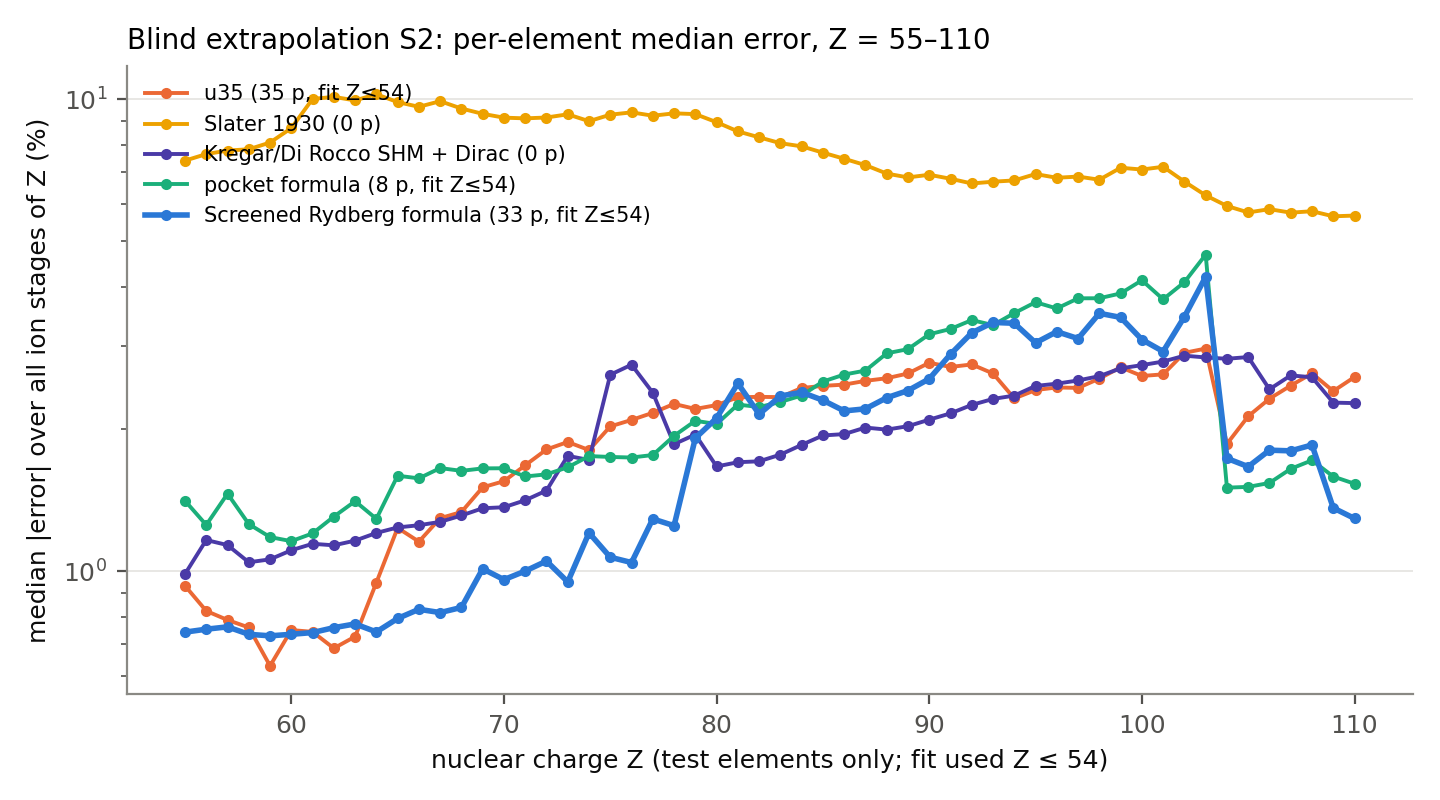
\includegraphics[width=0.75\columnwidth]{paper_blind_s2_by_Z.png}
\caption{Blind extrapolation. Each point is the median absolute percentage error over all ion stages of one element Z = 55–110. The three fitted models are fitted on Z ≤ 54 only; Slater's rules and the Kregar/Di Rocco SHM have no fitted parameters. The S2 MAPEs, computed from refits with the project's validation code, reproduce Table I (final 6.603 \%, u35 57.233 \%, pocket 11.334 \%, Slater 11.638 \%).}
\end{figure}

\begin{figure}[htbp]
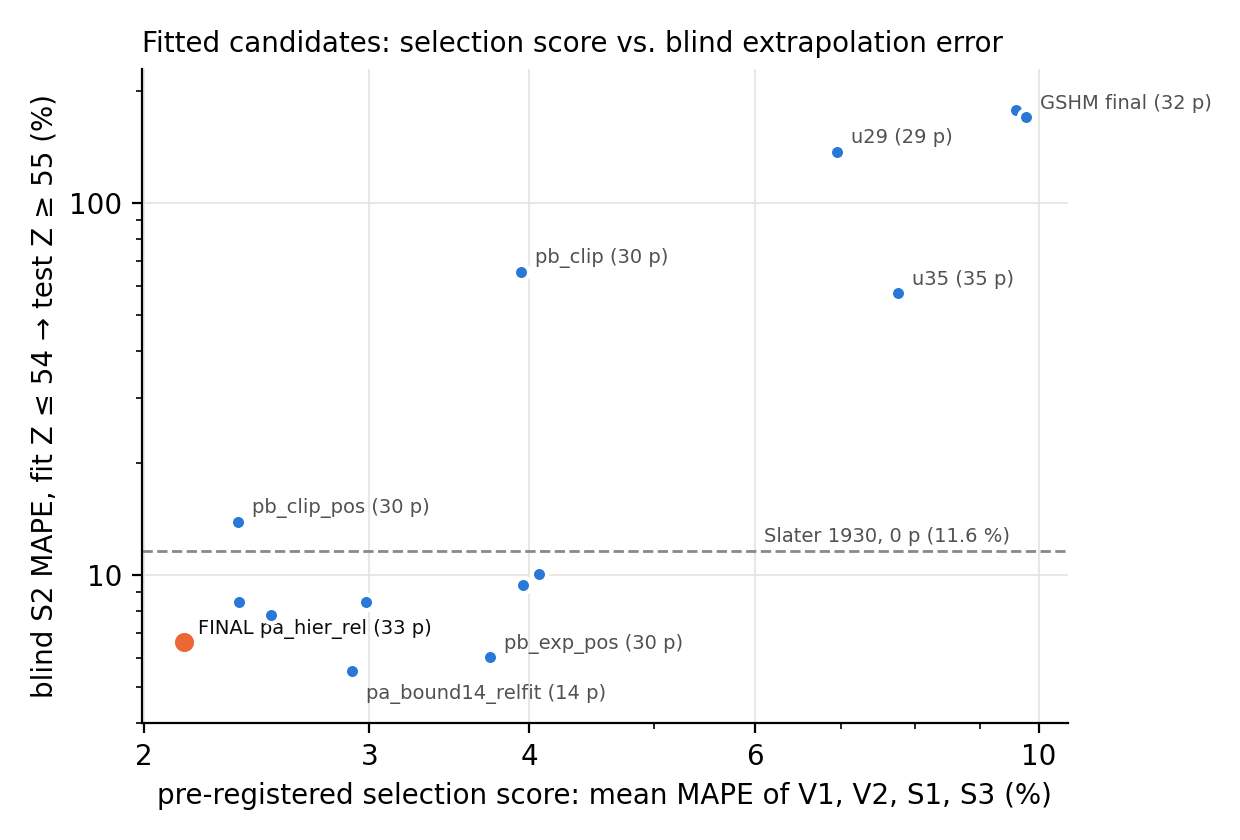
\includegraphics[width=0.75\columnwidth]{paper_selection_vs_blind.png}
\caption{Selection score (mean of V1, V2, S1, S3; no S2 data, although S1 and S3 contain Z ≥ 55 rows) against blind S2 MAPE for every fitted candidate in \texttt{results/model\_comparison.csv}. The pocket formula is omitted because its V1 fit diverged in the frozen run; that divergence depends on the optimizer path (Sec. III D), and with the converged V1 its selection score would be 4.19. The dashed line is Slater's rules (0 parameters).}
\end{figure}

The blind fit has three clear failures, which we report and have not corrected, since a correction now would be post hoc. Heavy p-block neutrals come out far too low (\texttt{results/known\_failures.json}, refit on Z ≤ 54): Pb at 1.20 eV against 7.42 eV, Tl at 1.74 against 6.11 and Rn at 6.10 against 10.75. The frozen run gave 1.19 and 1.73; refits in the two software environments differ here by about 0.01 eV. Lr comes out at −3.33 eV: the fitted r\_c are negative and the relativistic bracket is not bounded, so the Z\_eff bound alone does not keep the IE positive once Zα is large. Third IEs of lanthanides and actinides (4f/5f removal) are about 2.0–2.5 times too high (mean 2.2, median 2.1, 23 rows; worst Er²⁺ at 55.65 eV against 22.7 eV), because the Z ≤ 54 training set contains no f electrons.


\subsection{Hydrogen-like ions: correction layers}

\begin{table*}[htbp]
\caption{110 H-like ions, Z = 1–110 (\texttt{docs/first\_principles.md} §2.1).}
\footnotesize
\begin{ruledtabular}
\begin{tabular}{llll}
layer & MAPE (\%) & median (\%) & max (\%) \\
\hline
Bohr Ry Z² & 6.0 & 4.2 & 19.5 \\
(a) Dirac, point nucleus & 0.190 & 0.118 & 0.91 \\
(b) + recoil + finite nuclear size & 0.113 & 0.109 & 0.248 \\
(c) + one-loop QED (Uehling computed; F\_SE from [31]) & 0.00117 & 0.000154 & 0.0096 \\
(d) as (c) but with the closed-form Zα expansion of F\_SE & 0.354 & 0.191 & 1.18 \\
\end{tabular}
\end{ruledtabular}
\end{table*}


The NIST H-like reference values are themselves computed from the same QED theory, so layer (c) shows consistency with that source rather than independent validation. The remaining 10⁻⁵–10⁻⁴ residual at high Z is the omitted two-loop QED, nuclear-polarisation and recoil-QED terms.


\subsection{Head-to-head with published screened hydrogenic models}

We could specify two published SHMs fully from articles we were able to read: the parameter-free Kregar/Di Rocco model~\cite{r20,r22}, implemented from its definitions, and the relativistic model of Mendoza et al.~\cite{r16}, implemented from its published 19 × 19 table of fitted screening constants. The constants of More~\cite{r11} and of Faussurier et al.~\cite{r12} are in papers we could not access, and we found no verifiable reprint of their tables. We did not reconstruct them from memory.


\subsubsection{Kregar/Di Rocco SHM (parameter-free; all 5847 rows)}

Our implementation follows the published definitions: screening from hydrogenic densities with an exchange correction, iterated to self-consistency; energies E = −Σ q\_i Z\_i²/2n\_i²; and non-relativistic, Pauli and Dirac variants. Its same-shell Z → ∞ screening constants reproduce every printed digit (e.g. 1s 0.3125, 2p 0.3492), and its total energies agree with the published table within 0.71 \%. Its cross-shell constants differ by 0.011 on average (at most 0.053), because the original uses fitted closed forms whose coefficients we could not obtain~\cite{r19}. Valence IEs of near-neutral ions come out 3–5 eV higher than the printed model values; for Ar I we get 18.96 eV against 14.72 eV printed. Our near-neutral numbers therefore describe the model as defined, not the authors' code.


\begin{table*}[htbp]
\caption{Same 5847 rows, same scorer, MAPE in \% (\texttt{results/lit\_comparison.md}). For the 0-parameter models the S2 column is the error on the Z ≥ 55 rows; for the fitted models it is the blind S2 refit.}
\footnotesize
\begin{ruledtabular}
\begin{tabular}{lllllll}
model & params & all (median) & neutral 1st IE & H-like & charge ≥ 3 & S2 (Z ≥ 55) \\
\hline
Kregar/Di Rocco SHM, non-relativistic & 0 & 13.6 (2.34) & 230 & 6 & – & 15.1 \\
Kregar/Di Rocco SHM + Pauli & 0 & 12.6 (1.79) & 225 & 1.16 & – & 13.9 \\
Kregar/Di Rocco SHM + Dirac & 0 & 12.5 (1.71) & 224 & 0.19 & 4.68 & 13.6 \\
Slater 1930 & 0 & 11.8 (7.48) & 51.8 & 6 & 10.2 & 11.6 \\
pocket formula & 8 & 4.68 (3.04) & 16.8 & 1.16 & – & 11.3 \\
\textbf{final} & \textbf{33} & \textbf{1.87 (0.94)} & \textbf{7.52} & \textbf{0.0012} & \textbf{1.61} & \textbf{6.6} \\
\end{tabular}
\end{ruledtabular}
\end{table*}


Because of the valence discrepancy above, the 224 \% neutral-atom figure probably overstates the error of the authors' own model on neutral atoms. The parameter-free SHM works well for ionised species, with a median of 1.54 \% for charge ≥ 3. It fails near neutrality: 37 of its 5847 predictions are zero or negative, all for ions of charge 0–4 with an open d or f shell. Where the Z → ∞ limit dominates, parameter-free and exact-σ₁ models both work. Near neutrality every parameter-free hydrogenic model degrades, and the fitted remainder is what makes the formula useful there, at the price of 8–33 parameters. The bounded fitted formula extrapolates better (6.6 \%) than the parameter-free SHM scores on the same Z ≥ 55 rows (13.6 \%), while the unbounded fitted models extrapolate worse (57 \% and 170 \%).


\subsubsection{Mendoza et al. 2011 (published constants; 5011 covered rows)}

We transcribed the relativistic nlj screening constants of~\cite{r16} (the 19 × 19 matrix σ\_kk′, subshells 1s½ to 5p3/2) from Tables I and 2 of the authors' open-access deposit of the article (\url{https://oa.upm.es/11165/}), and implemented the model as published: Dirac energies of screened charges, Q\_k = Z − Σ\_k′ σ\_kk′(P\_k′ − δ\_kk′), and IE = E\_T(N−1) − E\_T(N) with NIST ground configurations. The implementation reproduces six of the paper's printed tables to their rounding, the 84 IEs of its Table III to ≤ 0.023 \% and its Tables IV–8 to ≤ 0.16 \% (\texttt{models/benchmarks/mendoza2011/}). We fitted no parameter.


Four caveats apply. The authors fitted the constants with a genetic algorithm to NIST and FAC energies of isoelectronic sequences from He to Eu, with Z up to 92, which overlaps our test rows, so no split is held out for this model. Neutral atoms and singly charged ions were excluded from their fit. The constants were optimised for ionization and excitation energies together, so an IE-only score is not what they were optimised for. And the tables stop at 5p3/2, so 836 rows (Z ≥ 55, ground configurations with 5d, 5f, 6s, 6p, 6d or 7s electrons) have no prediction. The comparison is therefore restricted to the 5011 covered rows.


\begin{table*}[htbp]
\caption{The 5011 rows covered by Mendoza et al.; same scorer, all three models fitted to all data (in-sample). Cells: mean / median absolute percentage error [n]. Source: \texttt{tools/compare\_mendoza.py} → \texttt{results/compare\_mendoza.md}.}
\footnotesize
\begin{ruledtabular}
\begin{tabular}{llll}
rows & Screened Rydberg (final, 33 p) & bounded 9-parameter (pa\_bound9) & Mendoza et al. 2011 \\
\hline
all covered rows & \textbf{1.62 / 0.78} [5011] & 2.63 / 1.19 & 2.82 / 0.85 \\
ions only (Z > N) & \textbf{1.55 / 0.76} [4957] & 2.54 / 1.17 & 2.56 / 0.82 \\
charge ≥ 3 & \textbf{1.45 / 0.73} [4837] & 2.43 / 1.14 & 2.27 / 0.77 \\
N ≤ 10 & 0.44 / 0.23 [1048] & 0.51 / 0.30 & \textbf{0.40 / 0.17} \\
11 ≤ N ≤ 36 & \textbf{1.43} / 0.82 [2275] & 2.12 / 1.17 & 1.82 / \textbf{0.61} \\
N ≥ 37 & \textbf{2.62 / 1.51} [1688] & 4.65 / 3.52 & 5.68 / 2.48 \\
Z ≥ 55 & \textbf{1.57 / 0.72} [3526] & 2.30 / 1.08 & 2.74 / 1.00 \\
H-like & \textbf{0.0012} [110] & 0.0012 & 0.19 \\
experimental & \textbf{4.37} [236] & 7.17 & 11.3 \\
neutral atoms (outside Mendoza's fit range) & 8.37 [54] & 11.5 & 27.1 \\
99th percentile / max APE & 11.3 / 30.4 & 14.8 / 38.0 & 28.4 / 119 \\
rows within 5 \% & 92.2 \% & 83.8 \% & 86.4 \% \\
\end{tabular}
\end{ruledtabular}
\end{table*}


On the ions it covers, the 33-parameter formula is competitive with the published constants of Mendoza et al., not decisively better. Its mean error is lower (1.62 \% vs 2.82 \%), its median is similar (0.78 \% vs 0.85 \%), and it has far fewer large misses (99th percentile 11 \% vs 28 \%). Mendoza et al. are more accurate for few-electron ions (N ≤ 10: 0.40 \% vs 0.44 \%) and have the lower median for 11 ≤ N ≤ 36. Row by row, the formula is closer to NIST on 51.3 \% of the covered rows. The 9-parameter variant matches their mean on ions (2.54 \% vs 2.56 \%) with a larger median.


The two models differ in size and scope. Mendoza et al. publish a 19 × 19 matrix with 331 non-zero constants, fitted by the authors; we count these as published numbers rather than independent degrees of freedom, and they are the only model-specific numbers our implementation of their IE prescription uses. The formula has 33 global parameters and was also validated on held-out splits. Their model also yields excitation energies and orbital properties and is used in plasma codes, while ours gives only ionization energies. The neutral-atom row lies outside the range they fitted and is shown for completeness. The experimental-row value here (236 rows) differs from the all-row value of Sec. III A (4.63 \% on 311 rows) only because the row sets differ.


A comparison with Dirac–Fock ionization energies~\cite{r30} on the same rows is left for future work.


\subsection{The exact first-order screening constants compared with Slater's}

\begin{table*}[htbp]
\caption{σ₁ for neutral-atom ground configurations, compared with Slater's σ. Excerpt; the full table for N = 1–110 is in \texttt{results/fp\_zexp\_coefficients.csv}, with values for all 5847 rows in \texttt{results/fp\_zexp\_rows\_coefficients.csv}.}
\footnotesize
\begin{ruledtabular}
\begin{tabular}{lllllll}
N & configuration & removed & E₁ (exact) & ΔE₁ & σ₁ (ab initio) & σ (Slater) \\
\hline
2 & 1s² & 1s & 5/8 & −0.625000 & 0.6250 & 0.30 \\
3 & 1s²2s & 2s & 5965/5832 & −0.397805 & 1.5912 & 1.70 \\
4 & 1s²2s² & 2s & 586373/373248 & −0.536469 & 2.1459 & 2.05 \\
6 & 1s²2s²2p² (³P) & 2p & 10957679/3359232 & −0.931338 & 3.7254 & 2.75 \\
8 & 1s²2s²2p⁴ & 2p & 4754911/839808 & −1.308370 & 5.2335 & 3.45 \\
10 & 1s²2s²2p⁶ & 2p & 2455271/279936 & −1.636495 & 6.5460 & 4.15 \\
11 & [Ne]3s & 3s & 9.635901 & −0.865071 & 7.7856 & 8.80 \\
18 & [Ne]3s²3p⁶ & 3p & 17.980333 & −1.407535 & 12.6678 & 11.25 \\
19 & [Ar]4s & 4s & 18.859971 & −0.879639 & 14.0742 & 16.80 \\
29 & [Ar]3d¹⁰4s & 4s & 39.317547 & −1.347129 & 21.5541 & 25.30 \\
36 & [Ar]3d¹⁰4s²4p⁶ & 4p & 50.145538 & −1.667284 & 26.6765 & 27.75 \\
\end{tabular}
\end{ruledtabular}
\end{table*}


E₁ is the Hund-term single-configuration value, except for N = 4 (Be), where σ₁ uses the Layzer-complex value 1.5592742. Decimal E₁ entries are exact rationals stored in the project cache, and σ₁ = −n²ΔE₁.


Slater's rules describe the neutral atom, while σ₁ is the exact screening in the bare-nucleus limit, and the two disagree in a systematic way (Fig. 3). For inner electrons the hydrogenic same-shell screening is stronger than Slater's 0.35 per electron (Ne 2p: 6.55 against 4.15). For valence electrons of heavy atoms σ₁ is much smaller than Slater's σ and than the screening implied by the measured IE (Na 3s: 7.79 against Slater 8.80 and an empirical 9.16; Cs 6s: 42.8 against Slater 52.8). The fitted remainder D supplies this difference near neutrality.


\begin{figure}[htbp]
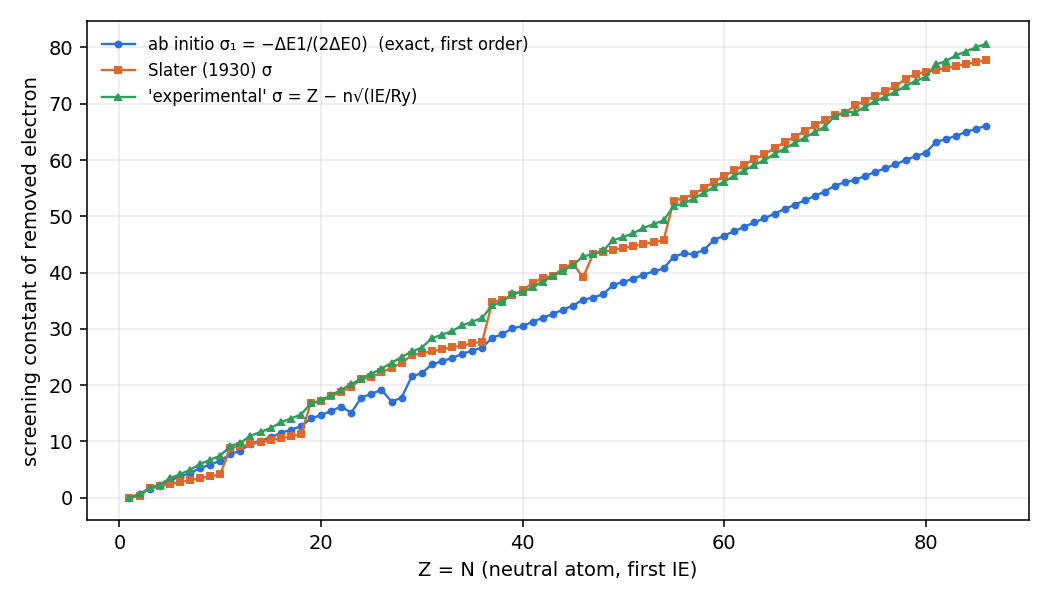
\includegraphics[width=0.75\columnwidth]{fp_sigma_abinitio_vs_slater.png}
\caption{Exact first-order screening σ₁ against Slater's σ for neutral-atom configurations.}
\end{figure}

\subsection{Worked examples and coverage}

For the first IE of oxygen (1s²2s²2p⁴ → 2p³, NIST 13.618 eV), σ₁ = 5.23348 and T = 3.3496. With h = 1.76652 this gives D = 0.71285 and Z\_eff = 2.05367, which lies between Z\_a = 1 and Z = 8. The hydrogenic term is 14.3457 eV, or 14.3162 eV after relativity, and the Hund term is −0.8365 eV, so IE = 13.479 eV, an error of −1.02 \%.


Nitrogen (1s²2s²2p³ → 2p², NIST 14.534 eV) has a half-filled shell. Here σ₁ = 4.37867 and T = 2.9470; with h = 1.62133, D = 0.63782 and Z\_eff = 1.98351. The hydrogenic term is 13.3822 eV, or 13.3626 eV after relativity. The Hund term is +0.8365 eV, since K\_p(3) = +1.2 has the opposite sign to oxygen's, and IE = 14.199 eV, an error of −2.31 \%.


For Mg²⁺ (NIST 80.144 eV) the formula gives 78.63 eV (−1.88 \%).


\begin{table*}[htbp]
\caption{Case studies: first IEs of six neutral atoms, with every intermediate quantity, for the three named models. Printed by \texttt{tools/audit\_components.py} and \texttt{tools/case\_study\_table.py} (\texttt{results/case\_studies.md}); the script asserts that the components reproduce the production code to 10⁻⁹. D is the screening remainder. The relativistic factor is F\_\{n,j\}·R for the σ₁ models (R = 1 for pa\_bound9) and the Sommerfeld bracket for the pocket formula.}
\footnotesize
\resizebox{\textwidth}{!}{%
\begin{tabular}{llllllllllllll}
\hline\hline
atom (removed) & model & σ₁ & ν\_g (same, in, core, df, out) & T & h & D & Z\_eff & Ry Z\_eff²/n² (eV) & rel. factor & Hund (eV) & IE (eV) & NIST (eV) & error \\
\hline
O (2p) & final & 5.2335 & 3, 4, 0, 0, 0 & 3.3496 & 1.7665 & 0.7128 & 2.0537 & 14.3457 & 0.99794 & −0.8365 & \textbf{13.479} & 13.618 & −1.02 \% \\
O (2p) & pa\_bound9 & 5.2335 & 3, 4, 0, 0, 0 & 3.0925 & 1.7665 & 0.6173 & 2.1492 & 15.7116 & 1.00002 & −1.4702 & \textbf{14.241} & 13.618 & +4.58 \% \\
O (2p) & pocket & – & 3, 4, 0, 0, 0 & – & – & 6.1394* & 1.8606 & 11.7747 & 1.00001 & −2.0735 & \textbf{9.701} & 13.618 & −28.76 \% \\
N (2p) & final & 4.3787 & 2, 4, 0, 0, 0 & 2.9470 & 1.6213 & 0.6378 & 1.9835 & 13.3822 & 0.99853 & +0.8365 & \textbf{14.199} & 14.534 & −2.31 \% \\
N (2p) & pa\_bound9 & 4.3787 & 2, 4, 0, 0, 0 & 2.8578 & 1.6213 & 0.5691 & 2.0522 & 14.3258 & 1.00001 & +1.4702 & \textbf{15.796} & 14.534 & +8.68 \% \\
N (2p) & pocket & – & 2, 4, 0, 0, 0 & – & – & 5.2632* & 1.7368 & 10.2598 & 1.00001 & +2.0735 & \textbf{12.333} & 14.534 & −15.14 \% \\
Na (3s) & final & 7.7856 & 0, 8, 2, 0, 0 & 7.1802 & 2.2144 & 1.1877 & 2.0266 & 6.2091 & 0.99905 & 0 & \textbf{6.203} & 5.139 & +20.70 \% \\
Na (3s) & pa\_bound9 & 7.7856 & 0, 8, 2, 0, 0 & 10.6892 & 2.2144 & 1.3219 & 1.8925 & 5.4142 & 1.00005 & 0 & \textbf{5.414} & 5.139 & +5.36 \% \\
Na (3s) & pocket & – & 0, 8, 2, 0, 0 & – & – & 8.9608* & 2.0392 & 6.2862 & 1.00006 & 0 & \textbf{6.287} & 5.139 & +22.33 \% \\
Ca (4s) & final & 14.6706 & 1, 8, 10, 0, 0 & 24.4604 & 4.3294 & 2.8939 & 2.4356 & 5.0444 & 0.99659 & 0 & \textbf{5.027} & 6.113 & −17.77 \% \\
Ca (4s) & pa\_bound9 & 14.6706 & 1, 8, 10, 0, 0 & 34.5745 & 4.3294 & 3.0747 & 2.2548 & 4.3233 & 1.00005 & 0 & \textbf{4.323} & 6.113 & −29.28 \% \\
Ca (4s) & pocket & – & 1, 8, 10, 0, 0 & – & – & 17.5935* & 2.4065 & 4.9248 & 1.00006 & 0 & \textbf{4.925} & 6.113 & −19.43 \% \\
Fe (4s) & final & 19.1852 & 1, 14, 10, 0, 0 & 30.9931 & 5.8148 & 3.8109 & 3.0039 & 7.6732 & 0.99190 & 0 & \textbf{7.611} & 7.902 & −3.69 \% \\
Fe (4s) & pa\_bound9 & 19.1852 & 1, 14, 10, 0, 0 & 38.1569 & 5.8148 & 3.8852 & 2.9296 & 7.2983 & 1.00009 & 0 & \textbf{7.299} & 7.902 & −7.64 \% \\
Fe (4s) & pocket & – & 1, 14, 10, 0, 0 & – & – & 22.8597* & 3.1403 & 8.3855 & 1.00011 & 0 & \textbf{8.386} & 7.902 & +6.12 \% \\
Pb (6p) & final & 63.7240 & 1, 20, 60, 0, 0 & 153.9342 & 17.2760 & 13.1422 & 5.1339 & 9.9612 & 0.79963 & +0.0465 & \textbf{8.012} & 7.417 & +8.02 \% \\
Pb (6p) & pa\_bound9 & 63.7240 & 1, 20, 60, 0, 0 & 189.5551 & 17.2760 & 13.3197 & 4.9564 & 9.2843 & 1.00019 & +0.0817 & \textbf{9.368} & 7.417 & +26.31 \% \\
Pb (6p) & pocket & – & 1, 20, 60, 0, 0 & – & – & 76.6038* & 5.3962 & 11.0052 & 1.00023 & +0.1152 & \textbf{11.123} & 7.417 & +49.97 \% \\
\hline\hline
\end{tabular}}
\end{table*}


*Pocket formula: total screening Σ s\_g ν\_g + t(N−1)/(Z\_a+κ); it has no σ₁ and no bound.


For s removal (Na, Ca, Fe) the IE is the screened Rydberg term times relativistic factors within about 1 \% of unity; no model in this paper adds an s-type correction. The final model is the most accurate of the three on O, N, Ca, Fe and Pb, pa\_bound9 only on Na, and the pocket formula on none. Both bounded models fail on Ca (−17.8 \% and −29.3 \%). For Pb, σ₁ = 63.72 (Fig. 3), while the total screening σ₁ + D is 76.87.


We evaluated the public API for every Z = 1–118 and every N = 1–Z, 7021 values. All are finite and positive, with no crashes. There are 22 violations of the monotonicity IE(Z, N−1) > IE(Z, N): 6 at Pt–Bi, caused by 4f/5s ordering, and 16 at Rf–Ds, where the input ground configuration jumps between neighbouring ions (e.g. Rf N = 68 is 4f¹²6s² and N = 69 is 4f¹⁴5d¹).


Above Z = 110 the predictions are qualitative. The 7p neutrals come out too low: Og is predicted at 3.66 eV, far below its lighter congener Rn (NIST 10.75 eV), again because of the negative r\_c.


\section{Discussion}

\subsection{What is new and what is rediscovered}

Much of the formula is known. The 1/Z expansion and its exact first-order term are Layzer's (σ₁ is his Z → ∞ screening constant~\cite{r4}), computed with textbook Slater-integral algebra~\cite{r33,r34}. The screened hydrogenic form goes back to~\cite{r1,r10,r11}, and self-consistent (Z, N)-dependent screening to~\cite{r17,r20}. The 1/(Z\_a + κ) remainder is Edlén-type isoelectronic behaviour~\cite{r8}. The one-electron Dirac, recoil, finite-size and QED corrections come from~\cite{r31,r32}, and LSDA ΔSCF from~\cite{r27,r28}.


Four things may be new. Z-expansion work~\cite{r4,r5,r9} computed first-order energies for selected configurations and isoelectronic sequences, and we are not aware of a table of exact first-order screening constants for every NIST ground configuration with N = 1–110; we offer ours as a complete tabulation, not as a new quantity. The formula joins exact σ₁ to a bounded fitted remainder in one closed form and is validated on all 5847 NIST successive IEs, with a pre-registered selection score and an extrapolation from Z ≤ 54 to Z ≥ 55; we found no out-of-range extrapolation test in the SHM literature we read. Two published SHMs are scored on the same rows: the Kregar/Di Rocco model on all 5847, and the constants of Mendoza et al. on the 5011 they cover, where the formula is competitive rather than decisively better (Sec. IV E). Finally, the 8-parameter pocket formula is a hand-calculable successor to Slater's rules, with 4.68 \% against 11.8 \% on all rows and 11.3 \% against 11.6 \% on blind S2.


We do not claim a first formula for all ionization energies, since SHMs and Dirac–Fock tables already cover all ions, or a first-principles formula, since only σ₁ and the one-electron corrections are first principles and the final model has 33 fitted parameters. We did not search the machine-learning literature on ionization energies systematically and make no claim relative to it.


Fitting alone interpolates to about 1.6 \% and extrapolates catastrophically (170 \%). Exact theory alone extrapolates smoothly but is about 70 \% off overall. Fixing the Z² and Z terms by theory and confining the fit to a bounded O(Z⁰) remainder gives about 2 \% inside the data and 6.6 \% in blind extrapolation.


\subsection{Where the formula fails}

Heavy near-neutral atoms, alkaline earths and noble gases are the main failure. The blind neutral first-IE MAPE is 21.8 \%, and the all-data neutral MAPE is 7.5 \% (6.4 \% for u35). Even with all data fitted (\texttt{results/known\_failures.json}) the ns² alkaline earths are too low (Ca −17.8 \%, Sr −14.8 \%, Ba −8.4 \%), Rn is too low by 24.6 \%, and Na is too high by 20.7 \% (Table VII). Pb's small all-data error (+8.0 \%) is partly a cancellation. Its Rydberg term alone is 9.96 eV (+34 \% against NIST 7.42 eV); the relativistic bracket, 0.80 because r\_p½ is negative, lowers it to 7.97 eV (+7.4 \%), and the final IE is 8.01 eV (Table VII; \texttt{results/audit\_components.md}). A term of the wrong physical sign is cancelling an overestimate. Valence screening in a neutral atom is an all-order, non-perturbative effect, and the parameter-free LSDA ΔSCF does better on neutral atoms (3.3 \% for Z ≤ 54).


The relativistic term is unbounded. The fitted r\_c are all negative (−0.45 to −1.47), opposite to the direct relativistic contraction of s and p½ electrons. Because the bracket is not bounded, the Z ≤ 54 fit gives a negative Lr and low superheavy 7p IEs. A bounded relativistic term chosen on V1/V2/S1/S3 alone is the obvious next step; the first attempt (Sec. III C) fixed the signs but lowered the selection score.


f-electron removal is the least accurate class, with 3.5 \% on all data and third IEs about 2.0–2.5 times too high (mean 2.2) in blind S2.


The formula has one Hund term per removed electron and no term-dependent multiplet energies, and ions whose ground configuration rearranges on ionization are described by single-configuration inputs. These limits also cause the 22 monotonicity violations.


19 of the 33 parameters are shrunk class deviations. The bounded 9-parameter variant pa\_bound9 (selection 2.51, blind S2 7.80 \%, all data 2.90 \%; parameters in Appendix A) is a reasonable alternative with fewer parameters, though it was not the pre-registered winner.


Most NIST values are labelled theoretical or semi-empirical (4617 + 919 of 5847), so agreement with them is partly agreement with other theory.


\subsection{Why no exact closed form exists for N ≥ 2}

With V = Σ 1/r\_ij the many-electron Schrödinger equation does not separate. E(Z) is analytic in 1/Z only up to a critical charge; for He, 1/Z\_c ≈ 1.0975. Beyond first order every coefficient E\_k (k ≥ 2) is an infinite sum over the hydrogenic continuum, with no known closed form even for two electrons, and is known only numerically~\cite{r6}. A closed formula for all ions must therefore combine exact low orders with an approximation for the rest. The choice is which approximation, and how it is validated. We keep the exact orders exact and confine the fit to the remainder, under a bound that prevents it from extrapolating wildly.


\section{Conclusions}

The screened Rydberg formula gives every successive ionization energy of every element from the configuration alone, with 33 global parameters. On 5847 NIST values its MAPE is 1.87 \% (median 0.94 \%), 7.5 \% for neutral atoms and 0.0012 \% for H-like ions. Fitted on Z ≤ 54, it predicts Z = 55–110 with 6.60 \% MAPE, below the 11.6 \% of Slater's rules and the 13.6 \% of a published parameter-free screened hydrogenic model, because first-order perturbation theory fixes the large-Z behaviour exactly and the fitted remainder is bounded.


The formula still fails in known places. In blind S2, Pb comes out at about 1.2 eV against 7.42 and Tl at about 1.7 eV against 6.11. Lr is negative in the Z ≤ 54 fit, and Og (3.66 eV) lies far below Rn. Alkaline-earth neutrals are too low, f-electron removal is too high in extrapolation, and all fitted relativistic coefficients are negative.


The most reusable result is the table of exact rational first-order screening constants σ₁ for N = 1–110.


\section*{Data and code availability}

All code, data and results are in the project repository, \url{https://github.com/AwaisSDev/Chem-Research}. It contains the NIST table (\texttt{data/nist\_ie.csv}) and the shared scorer (\texttt{evaluate.py}); the exact first-order coefficients (\texttt{results/fp\_zexp\_coefficients.csv}, \texttt{results/fp\_zexp\_rows\_coefficients.csv}); the final model and its parameters (\texttt{models/push\_a/model.py}, \texttt{models/unified/final.py}, \texttt{results/uni\_final\_params.json}); predictions for all rows (\texttt{results/uni\_predictions.csv}); the validation script (\texttt{models/unified/validate\_blind.py}); the literature re-implementations (\texttt{models/literature/kregar\_shm.py}, \texttt{models/benchmarks/mendoza2011/}); every per-row model input (\texttt{results/model\_inputs.csv}) with the stand-alone reference implementation (\texttt{tools/verify\_from\_inputs.py}), which reproduces the production predictions to 7·10⁻¹⁶; and the component audit (\texttt{tools/audit\_components.py}, Table VII) and benchmark matrix with row counts in every cell (\texttt{tools/benchmark\_matrix.py} → \texttt{results/benchmark\_matrix.md}). A command-line and Python interface (\texttt{ionization.py}) evaluates the formula for any Z ≤ 118 and N ≤ Z.


\begin{acknowledgments}
The computations, code, analysis and a draft of this text were produced with AI agents (Anthropic Claude) working under the author's direction. The author designed and directed the study and is responsible for the content. Every number in the paper is generated by a script in the repository and can be regenerated from it. Bibliographic data were checked against Crossref. No AI system is listed as an author.
\end{acknowledgments}

\appendix
\section{Fitted parameters (all-data fit)}

\begin{table*}[htbp]
\caption{Source: \texttt{results/uni\_final\_params.json}, which is identical to \texttt{results/pa\_params.json}.}
\footnotesize
\begin{ruledtabular}
\begin{tabular}{ll}
block & values \\
\hline
τ\_g (same, in, core, df, out) & 0.3928, 0.7879, 2.2243, 2.5488, 10.5688 \\
κ & 1.7527 (1.8027 as used in the code, which applies \textbar{}κ\textbar{} + 0.05) \\
δτ\_c (19 classes, defined in Table IX) & same\_s −0.1552, same\_p 0.0098, same\_d 0.0004, same\_f 0.1457, sn\_in\_p −0.1133, n1\_sp\_sp −0.3916, n1\_sp\_d 0.3009, n1\_sp\_f 0.2042, n2\_sp\_sp −0.2195, n2\_sp\_df −0.0622, d\_near −0.6962, n1\_d\_d −0.2689, n1\_d\_f 0.3286, f\_near 0.5476, n1\_f\_f −0.0918, out\_d −0.0176, out\_f 0.0173, core\_sp 0.2828, core\_df 0.1812 \\
r\_c (s, p½, p3/2, d, f) & −0.4543, −0.8129, −1.1533, −0.8426, −1.4672 \\
x\_l (p, d, f) & 0.2049, 0.4402, 0.4612 \\
\end{tabular}
\end{ruledtabular}
\end{table*}


**Bounded 9-parameter variant, pa\_bound9 (all-data fit, \texttt{results/pa\_params.json}, candidate \texttt{pa\_bound9}).** Same equation (2.2) and inputs as the final model, with T = Σ\_g τ\_g ν\_g (no class deviations), R = 1 (no relativistic bracket), and the same F\_\{n,j\}, μ and QED/FNS terms. Using these 4-decimal values instead of full precision changes no IE by more than 0.002 \% (\texttt{tools/hand\_recompute.py}).


\begin{table}[h]
\footnotesize
\begin{ruledtabular}
\begin{tabular}{ll}
block & values \\
\hline
τ\_g (same, in, core, df, out) & 0.2347, 0.5971, 2.9563, 2.9515, 23.7087 \\
κ & 2.2091 (2.2591 as used) \\
x\_l (p, d, f) & 0.3602, 0.4237, 0.8215 \\
\end{tabular}
\end{ruledtabular}
\end{table}


Metrics: all data 2.90 \% (median 1.39 \%), neutral 12.0 \%, H-like 0.0012 \%; V1 2.16, V2 1.95, S1 2.90, S3 3.05, selection score 2.51; blind S2 7.80 \% (Table I).


\begin{table*}[htbp]
\caption{Screening classes c and groups g of Sec. II B. (n, l) is the removed subshell and (n′, l′) the subshell of another electron. Each class lies inside one group. "rows" is the number of the 5847 NIST rows with ν\_c > 0. δτ\_c is from Table VIII, and τ\_g + δτ\_c is the coefficient of one electron of that class in T. (Verified by \texttt{tools/check\_grouping\_rule.py}.)}
\footnotesize
\begin{ruledtabular}
\begin{tabular}{lllllll}
group g & class c & target l & other electron (n′, l′) & rows & δτ\_c & τ\_g + δτ\_c \\
\hline
same & same\_s & s & (n′, l′) = (n, l) & 534 & −0.1552 & 0.2376 \\
same & same\_p & p & (n′, l′) = (n, l) & 1713 & 0.0098 & 0.4026 \\
same & same\_d & d & (n′, l′) = (n, l) & 1720 & 0.0004 & 0.3932 \\
same & same\_f & f & (n′, l′) = (n, l) & 717 & 0.1457 & 0.5385 \\
in & sn\_in\_p & p & n′ = n, l′ = s & 2073 & −0.1133 & 0.6745 \\
in & n1\_sp\_sp & s, p & n′ = n − 1, l′ = s, p & 2912 & −0.3916 & 0.3963 \\
in & n1\_sp\_d & s, p & n′ = n − 1, l′ = d & 1248 & 0.3009 & 1.0888 \\
in & n1\_sp\_f & s, p & n′ = n − 1, l′ = f & 386 & 0.2042 & 0.9921 \\
core & n2\_sp\_sp & s, p & n′ = n − 2, l′ = s, p & 2083 & −0.2195 & 2.0048 \\
core & n2\_sp\_df & s, p & n′ = n − 2, l′ = d, f & 668 & −0.0622 & 2.1621 \\
core & core\_sp & s, p & n′ ≤ n − 3 & 1311 & 0.2828 & 2.5070 \\
df & d\_near & d & n′ = n or n − 1, l′ = s, p & 1938 & −0.6962 & 1.8526 \\
df & n1\_d\_d & d & n′ = n − 1, l′ = d & 1078 & −0.2689 & 2.2799 \\
df & n1\_d\_f & d & n′ = n − 1, l′ = f & 391 & 0.3286 & 2.8773 \\
df & f\_near & f & n′ = n or n − 1, l′ = s, p, d & 778 & 0.5476 & 3.0964 \\
df & n1\_f\_f & f & n′ = n − 1, l′ = f & 201 & −0.0918 & 2.4569 \\
df & core\_df & d, f & n′ ≤ n − 2 & 2716 & 0.1812 & 2.7300 \\
out & out\_d & d & n′ > n & 15 & −0.0176 & 10.5512 \\
out & out\_f & f & n′ > n & 294 & 0.0173 & 10.5861 \\
out & sn\_out & any & n′ = n, l′ > l & 0 & none & 10.5688 \\
out & out\_sp & s, p & n′ > n & 0 & none & 10.5688 \\
\end{tabular}
\end{ruledtabular}
\end{table*}


**Pocket formula (8 parameters, all-data fit, \texttt{results/uni\_params.json}).** This is the only model called "pocket formula" in this paper.


\begin{equation}
Z_\mathrm{eff} = Z - \sum_g s_g\nu_g - t\,\frac{N-1}{Z-N+1+\kappa},\qquad
\mathrm{IE}=\mathrm{Ry}\,\frac{Z_\mathrm{eff}^2}{n^2}\Big[1+\frac{(Z_\mathrm{eff}\alpha)^2}{n^2}\Big(\frac{n}{j+\tfrac12}-\frac34\Big)\Big]+\mathrm{Ry}\,\frac{x\,K_l(k)}{n^2}
\end{equation}

The ν\_g are the five group counts of Sec. II B. The fitted values are s\_same 0.7499, s\_in 0.7514, s\_core 0.8432, s\_df 0.8408, s\_out 1.0497, t 1.3725, κ 9.815 (9.865 as used) and x 0.508.


\begin{thebibliography}{34}
\bibitem{r1} J. C. Slater, Atomic shielding constants, Phys. Rev. \textbf{36}, 57 (1930).
\bibitem{r2} E. Clementi and D. L. Raimondi, Atomic screening constants from SCF functions, J. Chem. Phys. \textbf{38}, 2686 (1963).
\bibitem{r3} E. Clementi, D. L. Raimondi, and W. P. Reinhardt, Atomic screening constants from SCF functions. II. Atoms with 37 to 86 electrons, J. Chem. Phys. \textbf{47}, 1300 (1967).
\bibitem{r4} D. Layzer, On a screening theory of atomic spectra, Ann. Phys. (N.Y.) \textbf{8}, 271 (1959), doi:10.1016/0003-4916(59)90023-5.
\bibitem{r5} D. Layzer, Z. Horák, M. N. Lewis, and D. P. Thompson, Second-order Z-dependent theory of many-electron atoms, Ann. Phys. (N.Y.) \textbf{29}, 101 (1964), doi:10.1016/0003-4916(64)90192-7.
\bibitem{r6} C. W. Scherr and R. E. Knight, Two-electron atoms III. A sixth-order perturbation study of the 1¹S ground state, Rev. Mod. Phys. \textbf{35}, 436 (1963), doi:10.1103/RevModPhys.35.436.
\bibitem{r7} A. Dalgarno and A. L. Stewart, A perturbation calculation of properties of the helium iso-electronic sequence, Proc. R. Soc. Lond. A \textbf{247}, 245 (1958), doi:10.1098/rspa.1958.0182.
\bibitem{r8} B. Edlén, Atomic spectra, in \emph{Handbuch der Physik}, Vol. 27, \emph{Spectroscopy I}, edited by S. Flügge (Springer, Berlin, 1964), pp. 80–220, doi:10.1007/978-3-662-35391-2\_2.
\bibitem{r9} U. I. Safronova, I. Yu. Tolstikhina, R. Bruch, T. Tanaka, F. Hao, and D. Schneider, Screening theory for transition energies of highly charged ions, Phys. Scr. \textbf{47}, 364 (1993), doi:10.1088/0031-8949/47/3/007.
\bibitem{r10} H. Mayer, \emph{Methods of Opacity Calculations}, Los Alamos Scientific Laboratory Report No. LA-647 (1947).
\bibitem{r11} R. M. More, Electronic energy levels in dense plasmas, J. Quant. Spectrosc. Radiat. Transf. \textbf{27}, 345 (1982), doi:10.1016/0022-4073(82)90127-3.
\bibitem{r12} G. Faussurier, C. Blancard, and A. Decoster, New screening coefficients for the hydrogenic ion model including l-splitting for fast calculations of atomic structure in plasmas, J. Quant. Spectrosc. Radiat. Transf. \textbf{58}, 233 (1997), doi:10.1016/S0022-4073(97)00018-6.
\bibitem{r13} G. Faussurier, C. Blancard, and P. Renaudin, Equation of state of dense plasmas using a screened-hydrogenic model with l-splitting, High Energy Density Phys. \textbf{4}, 114 (2008).
\bibitem{r14} P. Martel, J. G. Rubiano, J. M. Gil, L. Doreste, and E. Mínguez, Analytical expressions for the n-order momenta of charge distribution for ions, J. Quant. Spectrosc. Radiat. Transf. \textbf{60}, 623 (1998), doi:10.1016/S0022-4073(97)00226-4.
\bibitem{r15} J. G. Rubiano, R. Rodríguez, J. M. Gil, F. H. Ruano, P. Martel, and E. Mínguez, A screened hydrogenic model using analytical potentials, J. Quant. Spectrosc. Radiat. Transf. \textbf{72}, 575 (2002), doi:10.1016/S0022-4073(01)00142-X.
\bibitem{r16} M. A. Mendoza, J. G. Rubiano, J. M. Gil, R. Rodríguez, R. Florido, P. Martel, and E. Mínguez, A new set of relativistic screening constants for the screened hydrogenic model, High Energy Density Phys. \textbf{7}, 169 (2011), doi:10.1016/j.hedp.2011.04.006.
\bibitem{r17} M. Kregar, The virial and the independent particle models of the atom, Phys. Scr. \textbf{29}, 438 (1984), doi:10.1088/0031-8949/29/5/005.
\bibitem{r18} M. Kregar, The virial as the atomic model potential energy operator, Phys. Scr. \textbf{31}, 246 (1985), doi:10.1088/0031-8949/31/4/005.
\bibitem{r19} H. O. Di Rocco, Braz. J. Phys. \textbf{22}, 227 (1992), as cited in Ref.~\cite{r20} (not independently verified).
\bibitem{r20} J. Pomarico, D. I. Iriarte, and H. O. Di Rocco, An efficient screening approach to be used in plasma modeling and ion-surface collision experiments, Braz. J. Phys. \textbf{35}, 130 (2005), doi:10.1590/S0103-97332005000100008.
\bibitem{r21} F. Lanzini and H. O. Di Rocco, Screening parameters for the relativistic hydrogenic model, High Energy Density Phys. \textbf{17}, 240 (2015), doi:10.1016/j.hedp.2015.08.002.
\bibitem{r22} H. O. Di Rocco and F. Lanzini, Breit and quantum electrodynamics energy contributions in multielectron atoms from the relativistic screened hydrogenic model, Braz. J. Phys. \textbf{46}, 175 (2016), doi:10.1007/s13538-015-0397-9.
\bibitem{r23} B. F. Rozsnyai, Relativistic Hartree-Fock-Slater calculations for arbitrary temperature and matter density, Phys. Rev. A \textbf{5}, 1137 (1972), doi:10.1103/PhysRevA.5.1137.
\bibitem{r24} H.-K. Chung, M. H. Chen, W. L. Morgan, Yu. Ralchenko, and R. W. Lee, FLYCHK: Generalized population kinetics and spectral model for rapid spectroscopic analysis for all elements, High Energy Density Phys. \textbf{1}, 3 (2005).
\bibitem{r25} A. J. Crilly \emph{et al.}, SpK: A fast atomic and microphysics code for the high-energy-density regime, High Energy Density Phys. (2023), doi:10.1016/j.hedp.2023.101053.
\bibitem{r26} T. Koopmans, Über die Zuordnung von Wellenfunktionen und Eigenwerten zu den einzelnen Elektronen eines Atoms, Physica \textbf{1}, 104 (1934).
\bibitem{r27} W. Kohn and L. J. Sham, Self-consistent equations including exchange and correlation effects, Phys. Rev. \textbf{140}, A1133 (1965).
\bibitem{r28} S. Kotochigova, Z. H. Levine, E. L. Shirley, M. D. Stiles, and C. W. Clark, Local-density-functional calculations of the energy of atoms, Phys. Rev. A \textbf{55}, 191 (1997).
\bibitem{r29} S. J. Chakravorty, S. R. Gwaltney, E. R. Davidson, F. A. Parpia, and C. Froese Fischer, Ground-state correlation energies for atomic ions with 3 to 18 electrons, Phys. Rev. A \textbf{47}, 3649 (1993).
\bibitem{r30} G. C. Rodrigues, P. Indelicato, J. P. Santos, P. Patté, and F. Parente, Systematic calculation of total atomic energies of ground state configurations, At. Data Nucl. Data Tables \textbf{86}, 117 (2004), doi:10.1016/j.adt.2003.11.005.
\bibitem{r31} V. A. Yerokhin and V. M. Shabaev, Lamb shift of n = 1 and n = 2 states of hydrogen-like atoms, 1 ≤ Z ≤ 110, J. Phys. Chem. Ref. Data \textbf{44}, 033103 (2015).
\bibitem{r32} A. Kramida, Yu. Ralchenko, J. Reader, and NIST ASD Team, NIST Atomic Spectra Database (version 5.12) (National Institute of Standards and Technology, Gaithersburg, MD, 2024), \url{https://physics.nist.gov/asd}, doi:10.18434/T4W30F, accessed on or before 5 October 2026.
\bibitem{r33} R. D. Cowan, \emph{The Theory of Atomic Structure and Spectra} (University of California Press, Berkeley, 1981).
\bibitem{r34} C. Froese Fischer, T. Brage, and P. Jönsson, \emph{Computational Atomic Structure: An MCHF Approach} (Institute of Physics Publishing, Bristol, 1997).
\end{thebibliography}
\end{document}
